%================================================================
\section{On Generating Comics}

Skilled authors construct narratives in a way that facilitates their
comprehension by the audience. People learn to optimize their consumption of
relevant information~\cite{pirolli2007information}, and work to construct
inferences~\cite{magliano2016filling} about story content in the liminal spaces
of discourse (in between sentences in text, panels in comics, scenes in film);
inferences for story content are constructed when they are \emph{needed} for
comprehension, and \emph{enabled} by what has been narrated thus
far~\cite{myers1987degree}. All told, the dynamic between story authors and
consumers parallels the expected conduct of people engaged in cooperative
conversation as outlined by the philosopher of language \citeA{grice1975logic}.

For example, there 
exists a tacit expectation on behalf of story consumers that authors
will constrain their contributions to the discourse to what is relevant to
their narrative intent. As \citeA{murray2011why} states:
%
\begin{quote} 
	In a mature medium nothing happens, nothing is brought on stage (or screen 
	or comic book panel or described in prose) that does not in some way further 
	the action. Whatever the viewer is invited to direct attention to is
	something that further defines the role ([of a] character) or the function 
	(dramatic beat). 
	\end{quote}
%
These expectations give rise to narrative devices such as \emph{Chekhov's
gun}
and a related counterpart, the \emph{red herring}.
\note{CRM}{A red herring is a {\em violation} of such a principle, though
-- its purpose in discourse is to be uncooperative in the Gricean sense!
Is this worth mentioning, or just eliding the example?}

Thus, for the enterprise of computational narratology, it seems prudent to
encode the constraints and effects of narrative
discourse, since (as the primary point of contact with the narrative artifact)
narrative discourse carries with it expectations and conventions that
ultimately affect how story consumers understand the narrative. While we
acknowledge that coherent story structure is important for
comprehension~\cite{graesser2002how}, the narrative's meaning when read has
at least half to do with the cognition of the reader.
Story structure is recovered by the consumer insofar it is afforded by the
discourse structure. 

\note{CRM}{Somewhere in the below commentary, it would make sense to cite
~\cite{heider1944experimental}; I'm not sure where.}

{\em Purely visual comics}, or sequences of visual imagery arranged in
panels, present an excellent avenue along which to study discourse
theories computationally. 
The same principles apply: comprehensible comics
lack visual clutter, and differences across the {\em gutters} (gaps between
panels) are designed to be filled in by a reader's inference.
These principles, as well as notions of brevity, relatedness, and other
principles of cooperative narration, manifest in terms of discrete
particles that are easily recognized and generated by computer programs. 

Comics share structural similarity to written
text~\cite{saraceni2016relatedness}: they are both made up of individual
elements (sentences in text, panels in comics), delimited by special-purpose
symbols (full stops in text, panel borders in comics), which can be easily
identified, and which can contain a variable amount of information. However,
unlike text, comics afford an additional \emph{pictorial} dimension through
which to express information via a palette of visual elements and their spatial
relationships to one another, e.g. their relative size, rotation, horizontal and
vertical juxtaposition, and distance. While in general comics offer two
dimensions of authorship affordances (textual and visual language), in this work
we are concerned only with the pictorial dimension.

\citeauthor{saraceni2016relatedness} describes three notions of
\emph{relatedness} between comic elements.
Relatedness, a property of a comic that indicates how its panels are
connected or associated, depends on a comic's \emph{cohesion} -- the
lexico-grammatical features that tie panels together -- and \emph{coherence} --
the reader's perception of how individual panels contribute to her mental model
of the unfolding events. Relatedness emerges from a spectrum of \emph{textual}\footnote{\emph{Textual} here does not mean the use of actual text, but rather is a shorthand for \emph{surface code}~\cite{zwaan1998situation}.}
factors to \emph{cognitive} factors, illustrated in \fref{figure:relatedness}.
%
%\note{RCR}{It would be great to have one comic that allows us to talk about all three aspects.}
%

\begin{figure}
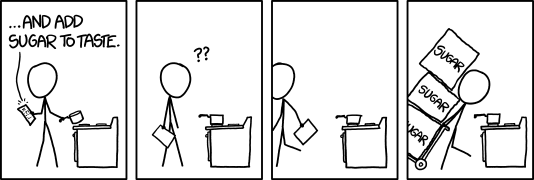
\includegraphics[width=0.5\textwidth]{xkcd-to_taste.png}
\caption{Strip \#1639 of {\em XKCD},
  \copyright Randall Munroe}
\label{fig:xkcd}
\end{figure}


\citeauthor{saraceni2016relatedness} distinguishes three categories of relatedness.
Closer to the textual end of the spectrum is the \emph{repetition} of visual
elements across panels. Beyond repetition is \emph{collocation}, which refers
to a reader's expectation that related visual elements will appear given the
ones that have been perceived. Closer to the cognitive end of the spectrum is
the \emph{closure} over comic elements, which refers to the way our minds 
complete narrative material given to us. Closure is terminologically borrowed 
from the field of visual cognition, but is intended as the mental process 
of inference that occurs as part of a reader's 
\emph{search for meaning}~\cite{gerrig1994readers}.

In Figure~\ref{fig:xkcd}, we see a comic that depends on all three aspects
of relatedness: first, repetition of the stove and pot is used to maintain
cohesion \note{CRM}{right term?} across panels. Second, the punchline of
the comic depends on collocation in the sense that we expect ``sugar'' to
come in small measurements, based on non-grammatical domain knowledge.
Finally, the comic depends on closure in that we expect the reader to infer
several things: that before the start of the comic, the character had been
following a recipe; that the character went to retrieve the boxes of sugar
between panels 3 and 4; and that the character intends to add sugar to the
pot.


%
\begin{figure}
	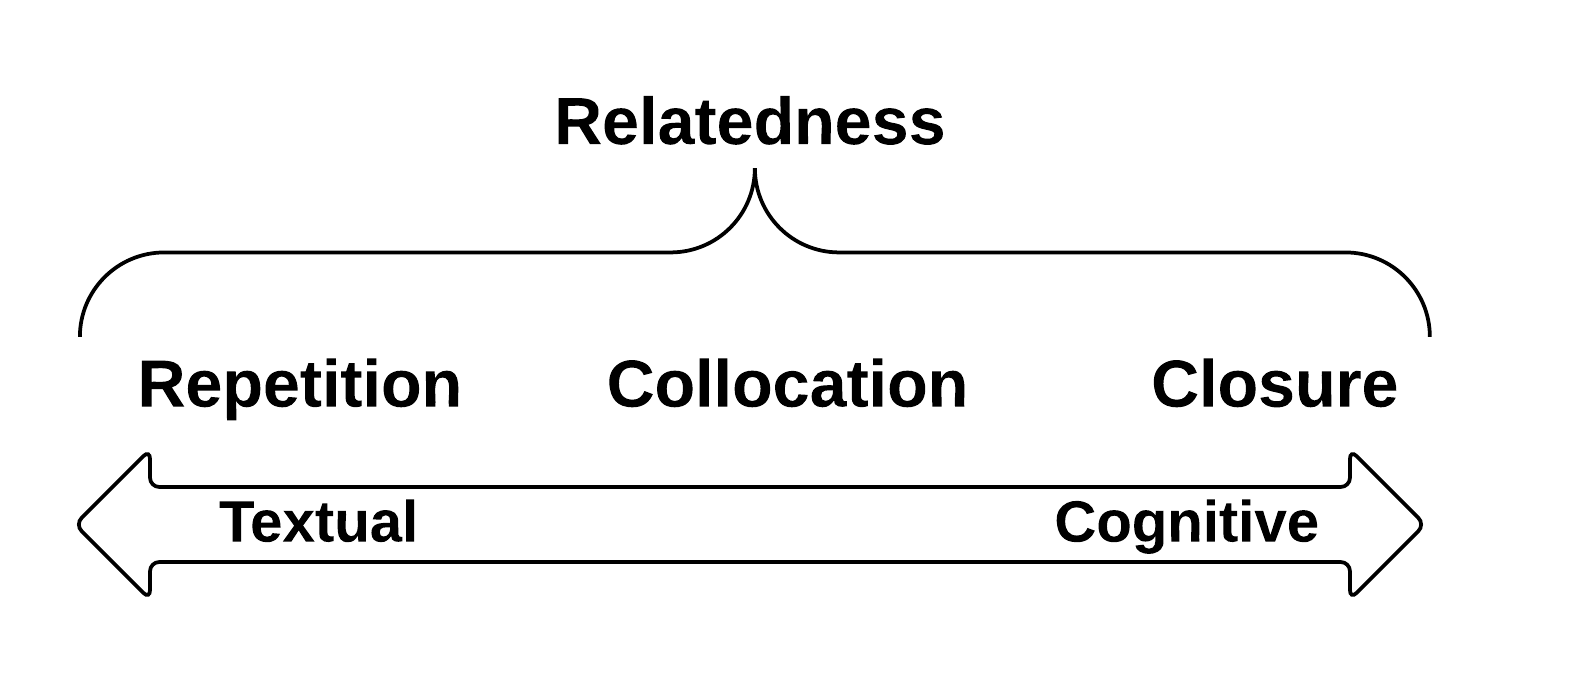
\includegraphics[width=\columnwidth]{relatedness.png}
	\caption{
		The spectrum of \emph{relatedness} as discussed by
		\citeA{saraceni2016relatedness}. Relatedness indicates how 
		comic panels are connected or associated in the minds of 
		readers, spanning from textual factors to cognitive factors. 
		Along that spectrum, there are three  distinguished 
		categories of relatedness: \emph{repetition}, 
		\emph{collocation}, and \emph{closure}, which have
		demonstrably different effects on the construction of
		narrative mental models.
		}
	\label{figure:relatedness}
\end{figure}
%
%	 	Indeed, \citeA{saraceni2016relatedness} argues that comic structure
%	 	ought to demonstrate \emph{relatedness}, which spans from the
%	 	structural aspects of discourse to the cognitive aspects of discourse
%	 	(which turns out to be the structural aspect of stories, needed for
%	 	sense-making).
%
% \note{RCR}{Discuss the three elements of Saraceni's account, including the closure principle (third aspect of \emph{relatedness}, which depends on not what is overtly explicit in the narrative's surface code, but also on inference. Borrowed from visual perception and Gestalt principles.}

%\note{RCR}{I think a figure that illustrates the spectrum of
%structural-relatedness to cognitive-relatedness would be good here.}
%
In our work we sought to develop a small scale computational model, and thus
focused primarily on modeling discourse structure which lies on the textual
side of the spectrum. However, our discourse model includes a minimal model of
story, which is needed in order to account for some elements of the cognitive
side of the spectrum.  We developed two computational models of discourse
structure: one based
on~\citeauthor{mcCloud1993understanding}'s~(\citeyear{mcCloud1993understanding})
account of \emph{transition types}, and the other based on
\citeauthor{cohn2013visual}'s~(\citeyear{cohn2013visual}) \emph{theory of visual
language}.


% Human brains' ability to fill in gaps is also why comics are simpler than
% animation in this respect: animations are expected to provide continuous
% motion between frames, whereas two comic frames need only be plausibly
% connected by some narrative justification. And that's where transition types
% come in: when you exclude non sequiturs, they constrain the space of next
% panels to ones that "make sense."

